%! Author = Saeid Yazdani
%! Date = 11/23/2023


\section{Product Lifecycle}
\label{sec:product-lifecycle}

As discussed in the last section, reliability, safety, and security are a set of
attributes that should exist not only at the design stage but ideally through
the whole operational lifetime of the system. The primary task of system
designers is to understand customer requirements well and develop and deliver
a system that presents the required functionality.
\autoref{fig:designer-idea-and-delivery} shows the different tasks during
product development and the quality assurance position within the development
flow.

\begin{figure}[htbp]
    \centering
    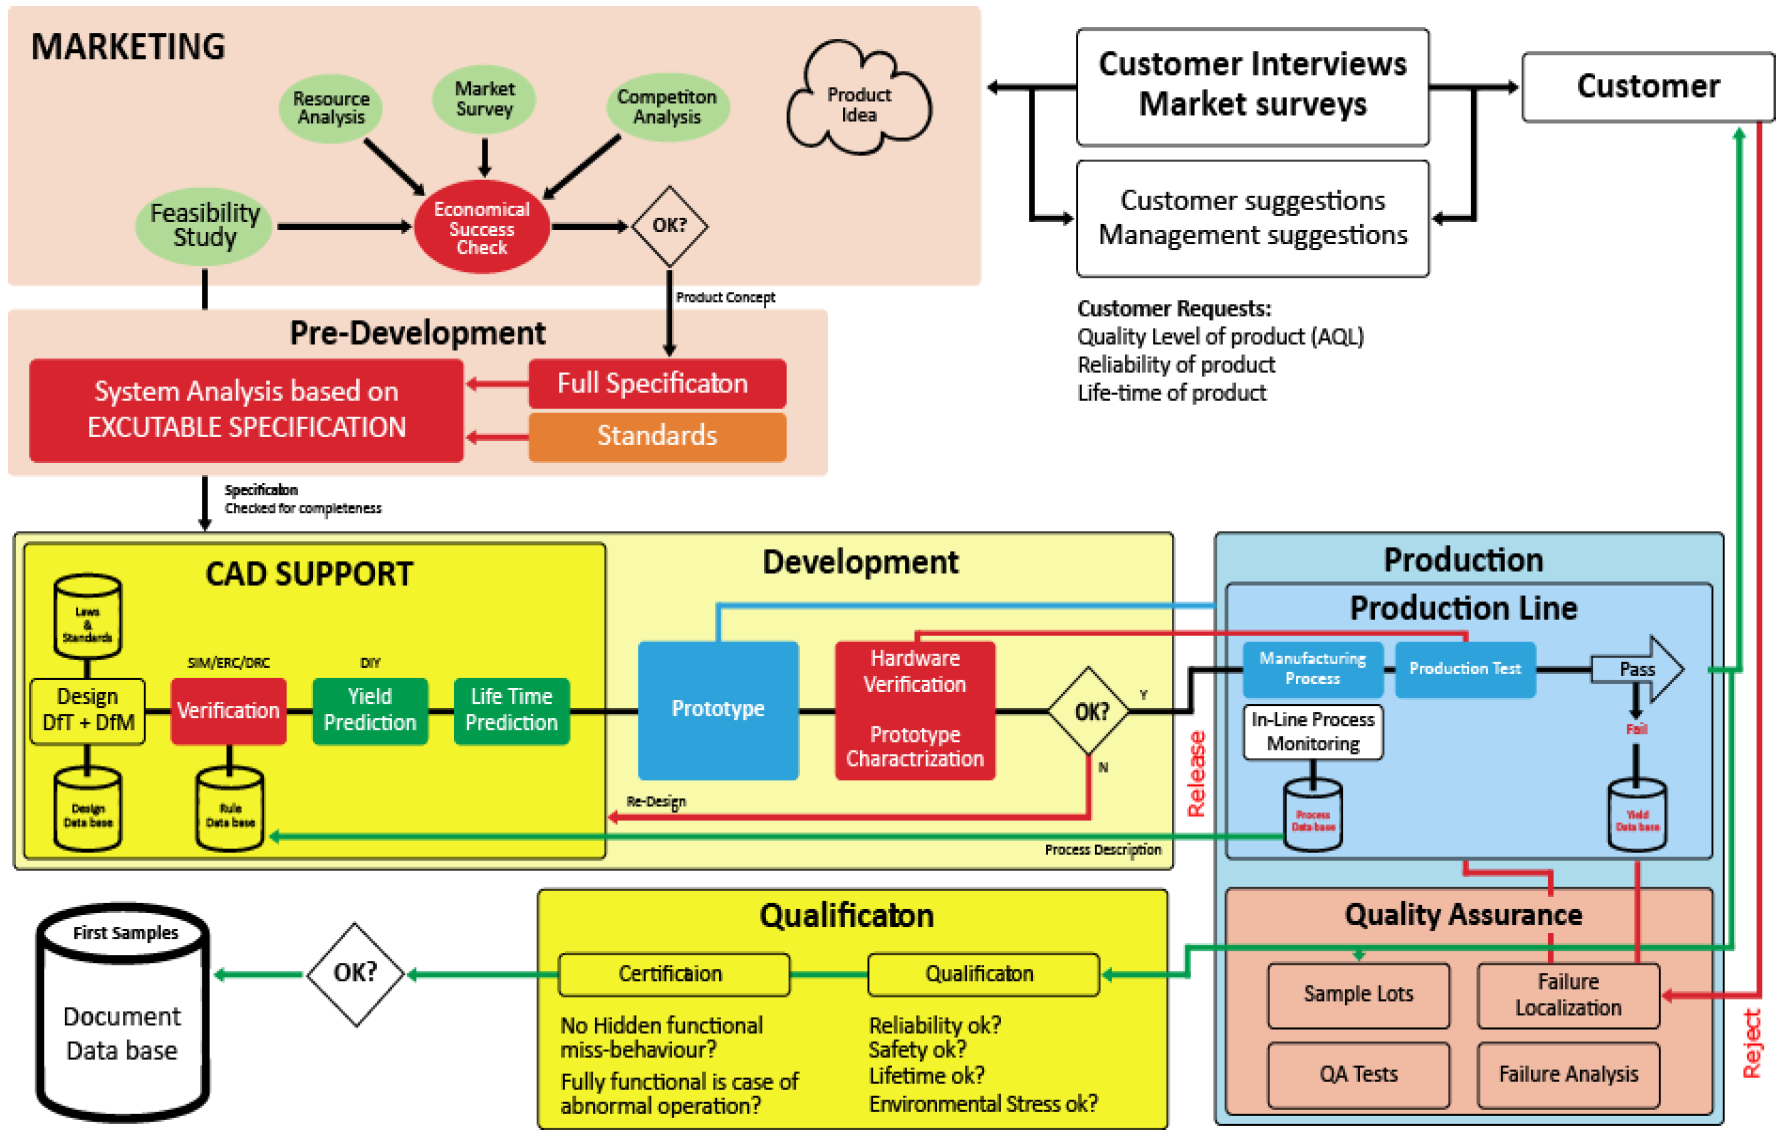
\includegraphics[width=\linewidth,height=0.62\textheight,keepaspectratio]
    {figures/designer-between-idea-and-product}
    \caption[Designer between idea and product delivery]
    {Designer between idea and product delivery.}
    \label{fig:designer-idea-and-delivery}
\end{figure}

Development of new products begins with marketing, where ideas are generated for
a specific application.
System designers are responsible for turning these concepts into reality, ensuring
not only that the product works as intended but also that it meets quality and cost
targets.
Customers expect full functionality, but additional requirements such as safety,
reliability, \ac{MTBF}, and \ac{SIL} must also be considered.
These aspects are often regulated or guided by standards, handbooks,
and design guides, which may be application-specific (e.g., nuclear, airborne,
automotive, or military standards).

The bottleneck between customers and designers is the different mindset or
business language.
Designers are technically oriented, and management is profit-oriented.
Often, design solutions are not accepted because of cost and time-to-market
factors.
Designers are constantly under pressure to deliver a product quickly and
cheaply.
They are sometimes forced to cut corners and use components or design
features different from what was initially determined.
This happens for various reasons:

\begin{itemize}[topsep=8pt,itemsep=4pt,partopsep=4pt, parsep=4pt]
    \item Time-to-Market/Competition timeline
    \item Final product cost and profit margin
    \item Market availability of components at the time of production
\end{itemize}

While developing a new product, we will always face the risk of misinterpreting
customer requirements.
A product is targeted towards a specific application area (automotive, airborne,
medical, industrial, commercial), and background rules are hidden behind these
application areas.
The designer must prove whether preliminary data meets the product
specifications.

This phase is called \emph{pre-development}, and preliminary studies, commonly
known as \emph{feasibility studies}, are carried out at this stage to help
designers and customers to measure and understand the practicality of the
design as a whole.
This calls for high-level analysis, and we refer to such tools as behavioral
verification tools, either based on CAD-based support that can analyze
specification completeness or by manual calculations (which is a tedious task).
High-level CAD tools for specification analysis have been around for decades,
but their acceptance is limited because operating such tools is still complex.
There are several views on a design based on legal issues. A product must be:

\begin{enumerate}[topsep=8pt,itemsep=4pt,partopsep=4pt, parsep=4pt]
    \item \textbf{\emph{Safe}:} Enforced by law.
    The designer must identify and mitigate any hazards associated with the product.
    All potential risks should be known and addressed before development begins.

    \item \textbf{\emph{Compliant}:} Enforced by law and standards.
    A product must meet all applicable regulations and standards, including limits on electromagnetic emissions, susceptibility to external disturbances (e.g., cosmic radiation in avionics), environmental rules, and industry-specific certifications (e.g., CE marking, ISO standards).

    \item \textbf{\emph{Reliable}:} Enforced by contract.
    Reliability ensures the product performs its intended functions consistently under specified conditions.
    Analysis typically covers fault tolerance, error rates, and maintainability. Lifetime may be part of contracts, but the focus is on predictable operation.

    \item \textbf{\emph{Secure}:} Enforced by law, contract, and best practices.
    Security protects against unauthorized access, data breaches, and tampering.
    Legal requirements, contractual obligations, and best practices define the needed measures. Poor security can lead to legal, financial, and reputational consequences.

    \item \textbf{\emph{Satisfying}:} Enforced by customer requirements.
    The product should meet user expectations and requirements.
    Usability, robustness, and user experience are key, including mechanical interfaces (buttons, displays) and \acp{GUI}. Even technically correct hardware may fail if the user interface is unintuitive or error-prone.
\end{enumerate}
